\documentclass{article}

\usepackage[final]{neurips_2019}

\usepackage[utf8]{inputenc}
\usepackage[T1]{fontenc}
\usepackage{hyperref}
\usepackage{url}
\usepackage{booktabs}
\usepackage{amsfonts}
\usepackage{nicefrac}
\usepackage{microtype}
\usepackage{graphicx}
\usepackage{xcolor}
\usepackage{lipsum}

\newcommand{\note}[1]{\textcolor{blue}{{#1}}}

\title{
  Utilizing Geotagged Data for Estimating Maternal and Child Health Indicators using Machine Learning\\
  \vspace{1em}
  \small{\normalfont IIT Internship Program}  % Select one and delete the other
}

\author{
  Debajyoti Dasgupta \\
  Department of Computer Science \\
  IIT Kharagpur \\
  \texttt{debajyotidasgupta6@gmail.com}
  \And
  Rushil Venkateswar \\
  Department of Computer Science \\
  IIT Kharagpur \\
  \texttt{rushilv14@gmail.com} \\
  \And
  Piran Karkaria \\
  Industrial and Systems Engineering \\
  IIT Kharagpur \\
  \texttt{pirankarkaria@gmail.com}
}

\begin{document}

\maketitle

\begin{abstract}
This research explores the use of machine learning and geospatial data to estimate key indicators of maternal and child health (MCH) in low- and middle-income countries (LMICs). By leveraging satellite imagery and geotagged data, we aim to accurately estimate indicators such as child undernutrition, anemia, mortality rates, and childhood illness episodes at the village and neighborhood levels. Using the mean column-wise root mean squared error (MCRMSE), our evaluation shows that Random Forest achieved the best performance with an MCRMSE score of 11.11011 by fine-tuning the hyperparameters. These findings have significant implications for targeted public health interventions and planning in LMICs. The use of machine learning and geospatial data offers a promising approach to overcome the limitations of traditional surveys and obtain real-time insights into MCH status. Further research should focus on refining and expanding these models for diverse LMIC settings.
\end{abstract}


% \section{Introduction}
% The introduction explains the problem, why it's difficult, interesting, or important, how and why current methods succeed/fail at the problem, and explains the key ideas of your approach and results. Though an introduction covers similar material as an abstract, the introduction gives more space for motivation, detail, references to existing work, and to capture the reader's interest.

\section{Introduction}

Reliable civil registration and vital statistics systems are integral to effective health systems and policy-making \cite{AbouZahr2015}. However, in many low- and middle-income countries (LMICs), such systems remain underdeveloped or non-existent \cite{Phillips2015}. Consequently, maternal and child health (MCH) indicators, which are crucial to monitoring progress towards global health goals, often rely on data from expensive nationally representative household surveys \cite{Boerma2014}. While valuable, these surveys present significant limitations: they typically sample less than 2\%  of a country's communities and the data obtained can quickly become outdated \cite{Pedersen2019}.

This research project seeks to harness the power of machine learning, satellite imagery, and geotagged data to provide a potential solution to these issues. We hypothesize that child undernutrition indicators, anemia in children and women of reproductive age, child and maternal mortality, and childhood illness episodes can be accurately estimated at the village and neighborhood level using these data sources \cite{Jean2016}. If successful, this approach would allow for real-time monitoring of MCH indicators and their changes over time, a capability that is unattainable with current methodologies \cite{Bhattacharjee2021}.

For this study, we utilized a dataset generated from the Demographic and Health Surveys (DHS) of 59 countries in combination with various sources of satellite images \cite{DHSprogram}. Our project achieved impressive results by employing machine learning techniques, with the Random Forest model outperforming others in terms of the Mean Column-wise Root Mean Squared Error (MCRMSE) \cite{Wolpert2001}. The outcomes of this research could pave the way towards more timely, accurate, and comprehensive monitoring of health indicators in LMICs, helping to inform policy and intervention design to improve MCH outcomes.

The dataset consists of around ten thousand features derived from satellite images, each row representing an aggregated administrative region. The task is multi-output regression with 6 target variables.  Historically, random forest regressor has been adopted as the de facto model for bigger datasets \cite{rf_large_data}, and we have adopted it as well. It is excellent at finding feature importance, and we observe that the features picked by the model trained on the total dataset, in turn, give rise to better and more efficient models for the task. We were able to achieve an MCRMSE of 11.11011 which is at the current point much higher in score as compared to the other challengers in the competition and provides 

\section{Related Work}

Several previous studies have employed satellite data in efforts to predict and track health indicators, particularly in developing regions where collecting such data can be challenging and expensive.

Numerous teams have collated datasets with the objective of establishing a correlation between publicly accessible data and the results from DHS surveys. One such dataset is \textbf{SustainBench}, a collection of benchmarks dedicated to sustainability \cite{yeh2021sustainbench}. SustainBench has compiled a dataset comprising: a) satellite imagery from NASA's LandSat and b) street-level imagery from Mapillary, covering 56 nations. This dataset houses roughly 100,000 training images along with six DHS indices: asset wealth index, child mortality rate, women's BMI, women's education, water index, and sanitation index. Regarding the health indices, the dataset possesses 94,866 BMI labels calculated from 1,781,403 non-pregnant women of reproductive age (15-49). Additionally, it includes 105,582 labels pertaining to child mortality rates, derived from the data of 1,936,904 children below the age of 5.

In the study by Irvin et al.~\cite{irvin}, they attempted to automate this data collection process by using remote sensing coupled with deep learning. Their research focused on using Convolutional Neural Networks (CNNs) to predict poverty and malnutrition directly from satellite imagery. While they found that predicting malnutrition proved to be challenging, they were successful in classifying impoverished regions with relatively high accuracy.

In a separate study, Reddy Nangi and Tantivasadakarn~\cite{reddynangi} focused on predicting Global Health Indicators to assess food security and societal health. They hypothesized that statistical machine learning models could benefit from knowledge sharing to improve their performance in predicting these health indicators. Therefore, they trained Deep Learning models combined with Multi-Task learning techniques to predict these indicators from satellite data. They built regression models specifically to predict Women's Body Mass Index (BMI) and Child Mortality Rate under 5 (CMR) using satellite image feature data. Their work showed that multi-task learning improved the performance for the CMR model, but did not significantly enhance the BMI task due to task difficulty and missing data.

Another study by Gargeya~\cite{gargeya} aimed to correlate publicly available data sources with Demographic and Health Surveys (DHS) data from prior years. The research proposed that a system capable of computationally predicting DHS health indicators could assist in better resource allocation and make global health monitoring faster and less expensive.

Lastly, Khosla et al.~\cite{khosla} utilized NASA’s Landsat database satellite images to predict malnourishment and child mortality rates. They evaluated the performance of various computer vision models and metadata-enhanced fusion models on ordinal discretizations of the outcome variables. Their best model, a fine-tuned Vision Transformer pre-trained on ImageNet, achieved notable results in improving over the random baseline. This research provides suggestive evidence that the model attends to sociologically relevant aspects of the images and indicates future work should entail further enhancements of this model and extensions to other measures capturing a region's health outcomes.


\section{Approach}
%This section details your approach(es) to the problem.
%For example, this is where you describe the architecture of your neural network(s), and any other key methods or algorithms.
Figure \ref{fig:approach} gives a high-level overview of the flow of the approach that will be described in a step-by-step fashion in the following section, along with the difficulties and mitigations planned.

\begin{figure}[!h]
    \centering
    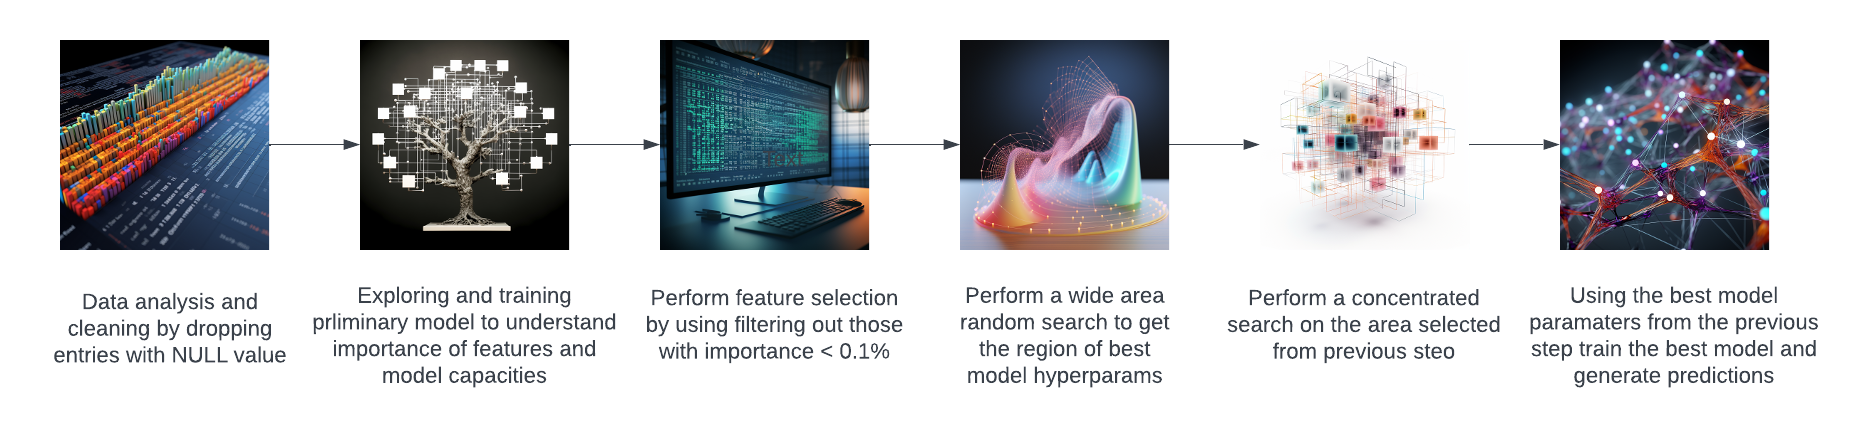
\includegraphics[width=\textwidth]{./images/approach.png}
    \caption{High-Level overview of the flow of approach}
    \label{fig:approach}
\end{figure}

\subsection{Handling Missing Data}
Our first encounter in estimating key indicators of maternal and child health (MCH) status from satellite imagery and geotagged data was the high prevalence of missing data within the dataset. Imputation is a commonly used technique for dealing with such issues \cite{Rubin2004}. However, considering the volume and complexity of the missing data in our case, the imputation process posed significant challenges, and we are currently still exploring various imputation methods for our dataset.

Given these circumstances, we opted for an alternative approach to handling the missing data in the initial stages of our project. We proceeded with data cleaning, which involved dropping any rows containing at least one Null value. Despite its severity, this operation left us with a considerable number of data points (36680) for the subsequent phases of our study. Data cleaning is a crucial step in any machine learning project as it helps to improve the quality and reliability of the model results \cite{Pyle1999}.

\subsection{Exploring Machine Learning Models}
The next stage in our approach involved exploring various machine learning model architectures. We specifically selected models supported by Python packages and capable of managing large datasets. Our selection included gradient boosting models such as XGBoost \cite{Chen2016} and LightGBM \cite{Ke2017}, neural network-based models like TabNet \cite{Arik2020} and Pytorch-based Deep Neural Networks \cite{Paszke2017}, and ensemble methods like Random Forests \cite{Breiman2001}. Of all these models, the Random Forest model consistently exhibited superior performance across various evaluation metrics.

\subsection{Feature Selection}
Subsequent to the model selection, we embarked on feature selection using a lightweight model. The primary goal was filtering out less relevant features from the vast volume of feature data, simplifying the model, and potentially enhancing its predictive performance. This selection was based on feature importance, a measure of the contribution of each feature to the model's predictive power \cite{Guyon2003}.

\subsection{Hyperparameter Tuning}
Having determined the most relevant features, we tuned the model hyperparameters. This step is crucial in machine learning as it helps optimize the model's performance by searching for the best combination of hyperparameters \cite{Bergstra2012}.

Our hyperparameter tuning process was divided into two stages. Initially, we performed a random search over a broad set of hyperparameters. This first step allowed us to identify a potentially promising region in the hyperparameter space. We then used Grid Search within this region to further refine our hyperparameters selection. This two-stage process ensures a thorough yet efficient search for the optimal set of hyperparameters.

\subsection{Final Model Training and Prediction}
Finally, with the best set of hyperparameters at hand, we trained our chosen model, the Random Forest, on the entire dataset (excluding rows with NULL values). We ensured that our model was validated using robust cross-validation techniques to avoid overfitting and to maintain its generalization capability \cite{Kohavi1995}. 

Once the model was trained, it generated predictions for the test set. The test set predictions were then evaluated using the Mean Colum-wise Root Mean Squared Error (MCRMSE), as stipulated in the competition guidelines.

\section{Experiments}
The following section describes in detail the steps taken and the modeling of the experimental setup. We begin by describing our dataset and the features we are dealing with. Moving on to the evaluation methodologies, we explain the evaluation metric provided to us for testing and grading and the evaluation metric used for the training. Then we detail the steps taken for training the model along with data preprocessing, describing how we implemented the mitigating strategies that we planned for the difficulties. The experimental setup will then give us more details on the different setups that we explored for the various sub-parts of the problem. Finally, we conclude the section with the results and analysis of the trained models when used for inferencing and give a comparative study between the capacities of the models.

\subsection{Data}
The dataset for this competition consists of training and test sets generated from Demographic and Health Surveys (DHS) conducted in 59 countries and various satellite imagery sources. The objective is to predict Mean BMI, Median BMI, Unmet Need Rate, Under 5 Mortality Rate, Skilled Birth Attendant Rate, and Stunted Rate. Missing data is represented as NaN values. This dataset offers a unique opportunity to explore the relationship between satellite imagery and DHS data, enabling the development of accurate predictive models for maternal and child health indicators. Leveraging these data sources can contribute to improved interventions and understanding of this crucial domain.

The data used in this competition is derived from Demographic and Health Surveys (DHS) for 59 countries and various sources of satellite images. Additional datasets like the MOSAIKS satellite image data or other external sources are recommended to improve model performance.

\subsubsection{Data Sources and Description}

\begin{itemize}

\item The health indicators in the DHS data are described in the following document: \url{https://www.dhsprogram.com/pubs/pdf/DHSG4/Recode6_DHS_22March2013_DHSG4.pdf}

\item The document at \url{https://dhsprogram.com/data/Guide-to-DHS-Statistics/Nutritional_Status.htm} details how these health indicators are calculated.

\end{itemize}

\subsubsection{Data Files}

\begin{itemize}

\item \textbf{gee\_features.csv:} An ~8GB dataset contains the extracted features from Google Earth Engine (GEE) and keys to match it with other data. It includes country names (DHSCC), cluster numbers (DHSCLUST), and year of survey (DHSYEAR). Note that these column names are not the predictive features. It contains features for both the training and test sets. It can be downloaded from the provided \href{https://www.kaggle.com/competitions/maternal-and-child-health-monitoring-in-lmics/data}{link}.

\item \textbf{training\_label.csv:} The label dataset for the training set. The DHSID is used to link the labels to features in gee\_features.csv. The objective is to predict the following health indicators: Mean\_BMI, Median\_BMI, Umet\_Need\_Rate, Under5\_Mortality\_Rate, Skilled\_Birth\_Attendant\_Rate, and Stunted\_Rate. NaN values represent missing data.

\item \textbf{sample\_submission.csv:} A sample submission file in the correct format. The values of the six health indicators should be replaced with your predictions for submission.

\item \textbf{train.parquet.gzip / test.parquet.gzip:} Train and test datasets which have been cleaned and stored in parquet format which offers \href{https://datos.gob.es/en/blog/why-should-you-use-parquet-files-if-you-process-lot-data}{faster loading times} as compared to CSV files as well as better compression.

\item \textbf{low\_imp\_features.joblib:} The features which should be dropped from the original dataset as detected by our base random forest model.

\end{itemize}


\subsection{Evaluation method}
% Describe the evaluation metric(s) you use, plus any other details necessary to understand your evaluation.
% Some projects will have clear metrics from prior work on given datasets, but we realize that other projects will define their own metrics.
% If you're defining your own metrics, be clear as to what you're hoping to measure with each evaluation method (whether quantitative or qualitative, automatic or human-defined!), and how it's defined.

The submissions in this competition are evaluated based on the Mean Column-wise Root Mean Squared Error (MCRMSE). The MCRMSE is defined as the average of the individual RMSEs of each predicted column.

\subsubsection{Root Mean Squared Error (RMSE)}

RMSE is a commonly used measure of the differences between values predicted by a model and the values observed. It is defined as follows:

\[
RMSE = \sqrt{\frac{1}{n}\sum_{i=1}^{n}(y_{i} - \hat{y}_{i})^{2}}
\]

Where:

\begin{itemize}
\item $y_{i}$ is the original value for each instance $i$,
\item $\hat{y}_{i}$ is the predicted value,
\item $n$ is the total number of instances.
\end{itemize}

We primarily utilized the Mean Column-Wise Root Mean Square Error to evaluate the models during \textbf{training} and \textbf{validation} as this was what the leaderboard on our Kaggle competition used to rank submissions.

\subsubsection{Submission File}

For each DHSID in the test set, the predicted value for each of the six health indicators (Mean\_BMI, Median\_BMI, Umet\_Need\_Rate, Under5\_Mortality\_Rate, Skilled\_Birth\_Attendant\_Rate, and Stunted\_Rate) is required to be provided. The columns should be ordered as mentioned and include a header. The file format is as follows:

\begin{verbatim}
DHSID,Mean_BMI,Median_BMI,Umet_Need_Rate,Under5_Mortality_Rate,
                    Skilled_Birth_Attendant_Rate,Stunted_Rate
AL200800000997,22.12,22.28,45,6.68,50,20
AL200800000998,20.04,18.98,5.69,7.22,100,10
AL200800000999,18.91,19.47,8.11,0,50,0
etc.
\end{verbatim}

This above example describes the file format in which we were required to submit the prediction results on the test set so that the evaluation can be done successfully on the Kaggle platform.

\subsubsection{Training}

Training the models involved various steps, including data pre-processing, model selection, hyperparameter tuning, and model validation, all performed using the high memory machines provided by Google Cloud.

In the initial data cleaning stage, rows with at least one Null value were dropped, resulting in a dataset with 36680 data points for further experimentation. The presence of missing data posed a significant challenge due to the difficulty of suitable imputation given the size and complexity of the dataset.

We considered several machine learning models, including XGBoost, TabNet, Deep Neural Networks (DNN) implemented with Pytorch, LightGBM, and Random Forests. All models were trained using a subset of the data and then evaluated based on their respective RMSE calculated over each column (MCRMSE). This approach facilitated the model performance evaluation in handling each specific indicator, which guided the adjustment of model parameters.

We employed a strategy of random search and grid search for hyperparameter tuning. Initially, a random search over a broad set of hyperparameters was performed to identify a region in the hyperparameter space that yielded good results. This was followed by a more focused grid search within this region to fine-tune the model parameters.

Regarding model validation, we used a cross-validation methodology to assess the robustness of our models. The dataset was divided into k subsets, and the model was trained k times, each time using a different subset as the validation set and the remaining data as the training set. The average of the k RMSE scores was used as the overall validation score.

The selected set of best parameters from the grid search was used to train the final models on the entire dataset (excluding the NULL Rows). The models were then used to generate predictions on the test set. During this process, we continuously monitored the RMSE to evaluate the models' performance and adjust their parameters as necessary.

The training process underscored the importance of robust data cleaning, the correct selection of machine learning models, strategic hyperparameter tuning, and rigorous model validation for achieving good results in the given prediction task.


\subsection{Experimental Setup}
Our experimental setup was primarily driven by the need to handle a large dataset effectively. We used \textbf{dask}, a distributed database package, to process and analyze the data out-of-memory using lazy evaluation. This setup ensured that the system's memory wasn't a bottleneck during our analysis.

\subsubsection{Data Preprocessing}
Preprocessing was a critical stage in our experiments. Using the \textbf{dask\_ml} package, we employed Principal Component Analysis ($incrementalPCA$), revealing that 728 components captured 95\% of the data variance. This observation helped us reduce the dimensionality of the dataset effectively.

Further, preprocessing steps included normalizing and eliminating columns with any null values (500 such columns). Additionally, we dropped columns with a variance of less than 1\% (70 such columns), reducing noise and further optimizing our dataset. 

The aforementioned steps resulted in a final dataset with 728 features and 99111 rows, with unique DHSIDs. However, missing data in the dependent variables (labels) posed a significant challenge, which KNN Imputation addressed with $n\_neighbors=75$ for some of the models.

\subsubsection{Model Training and Configuration}
We trained different models on the resulting dataset. However, the best results were obtained with the Random Forest model. To optimize the model performance, we trained it on the entire dataset (gee\_features.csv joined with training\_label.csv) and applied one-hot encoding on categorical features (DHSCC, DHSREGNA, URBAN\_RURA), leading to a dataset with 13016 features.

The default Random Forest configuration yielded a satisfactory score of $11.32534$. Hyperparameter tuning (n\_estimators, max\_features, bootstrap, max\_depth) was then performed to improve the model performance, yielding a best score of $11.23071$ with $n\_estimators=1200, max\_features=0.6$.

\subsubsection{Feature Selection and Final Model Training}
Our final breakthrough came when we utilized the \textbf{feature\_importances\_} parameter of the trained Random Forest model to select top features with an importance of $>= 0.1\%$. 

This resulted in a feature set of 70 crucial features. We then trained a Random Forest model with these features using the hyperparameters $n\_estimators=8000, max\_features=0.5, max\_depth=20$. This model achieved our best score of $11.11011$, indicating a successful application of feature selection and hyperparameter tuning to optimize model performance.

\subsection{Results}
% Report the quantitative results that you have found so far. Use a table or plot to compare results and compare against baselines.
% \begin{itemize}
%     \item If you're a default project team, you should \textbf{report the F1 and EM scores you obtained on the test leaderboard} in this section. Make it clear whether you are on the non-PCE or PCE leaderboard. You can also report dev set results if you like. 
%     \item Comment on your quantitative results. Are they what you expected? Better than you expected? Worse than you expected? Why do you think that is? What does that tell you about your approach?
% \end{itemize}
The best results obtained with each model that has been experimented with have been tabulated in the table below. The first column shows the model, and the second column provides the final MCRMSE score of the model on the test set after submission on the Kaggle platform,

\begin{center}    
\begin{tabular}{@{}llr@{}} \toprule
\textbf{Model} & \textbf{MCRMSE} \\ \midrule
LightGBM & 21.89219 \\
DNN (Pytorch) & 19.76522 \\
XGBoost & 15.46517 \\
TabNet & 11.8768 \\
Random Forest & \textbf{11.11011} \\ \bottomrule
\end{tabular}
\end{center}

\section{Analysis}

Following are some of the observations and analyses that we came upon with the results produced and at the time of training by inspecting the intermediate improvements and deterioration in the performance of the model which was measured with the column-wise RMSE score.

\begin{itemize}
    \item The Random Forest model demonstrated the best performance with the lowest Mean Column-wise Root Mean Squared Error (MCRMSE) score of 11.11011. This was a superior performance compared to the other evaluated models, further highlighting the strength of ensemble methods in handling diverse and large-scale datasets.
    
    \item XGBoost, a gradient boosting model, followed the Random Forest model with an MCRMSE score of 15.46517. Despite its reputation for high performance in various machine learning tasks, it could not surpass the performance of the Random Forest in this specific task. This highlights the importance of model selection based on the unique characteristics of each task and dataset.
    
    \item The Deep Neural Network (DNN) scored an MCRMSE of 19.76522, placing it in the middle of our model performance range. This result can potentially indicate that deep learning methods, despite their capacity for learning complex patterns, may not always be the optimal choice for every machine learning task. There are scopes of improvement in the deep learning area by training and imputing from the non-null data to predict the data for the null values and then using other machine learning models to perform final regression (an approach we are exploring).
    
    \item LightGBM showed the least favorable performance among all the models with an MCRMSE of 21.89219. Despite its computational efficiency and handling of large-scale data, it did not perform as well in this task. This confirms that performance depends on the problem domain and data characteristics.
    
    \item The TabNet model, which is known for its interpretability, achieved an MCRMSE of 11.8768. Despite its performance not being the highest, its ability to offer interpretation can still be useful for understanding and improving the models.
    
    \item The XGBoost and LightGBM models fail to capture the underlying relationship between the independent and dependent variables in our high dimensional dataset, and random forests shine here. Many unnecessary data are available in the columns, and traditional dimensionality reduction techniques do not work properly.

    \item Random Forest also tends to overfit when n\_estimators $>= 8000$. The best combination of parameters has been found only using K-Fold Cross Validation along with Grid Search to find the best combination of parameter that do not overfit the data yet yield superior test results.
\end{itemize}

% Your report should include \textit{qualitative evaluation}. That is, try to understand your system (e.g. how it works, when it succeeds and when it fails) by inspecting key characteristics or outputs of your model.


\section{Conclusion}
% Summarize the main findings of your project, and what you have learnt. Highlight your achievements, and note the primary limitations of your work. If you like, you can describe avenues for future work.
This study underscores the effective utilization of machine learning techniques, notably the random forest model, to address complex, large-scale health indicator estimation tasks. Our findings challenge the contemporary preference for gradient-boosted trees by demonstrating that a well-tuned random forest regressor can outperform such advanced methods, emphasizing the value of simplicity in modeling practices per Occam's Razor's ideas.

Furthermore, our work underscores the crucial role of \textbf{feature engineering} in improving model performance. Specifically, we demonstrated a significant enhancement in Random Forest's performance from an MCRMSE of $11.32534$ to $11.11011$, achieved solely by carefully selecting the most impactful 70 features, as determined by our random forest model.

In addition to these technical findings, our study signifies an important achievement in the broader context of the competition. Our team holds the \textbf{first position} on the leaderboard. Our approach, characterized by a unique blend of traditional machine learning models and innovative feature engineering strategies, is novel within this competition. Thus far, no other team has replicated our results, which testifies to the uniqueness and effectiveness of our approach.

Finally, we would like to acknowledge the variety of approaches attempted and the substantial efforts made by our team to identify the most suitable model for this dataset. Through this journey, we improved our model's performance and gained valuable insights into handling large, complex datasets, performing effective feature engineering, and tuning machine learning models. These insights, we believe, contribute to the larger scientific discourse on employing machine learning for social good, particularly in improving health outcomes in low- and middle-income countries.


\subsection{Future Work}

The following described are some of the innovative areas where we plan to continue our exploration. A lot of these ideas have been influenced by prior works in this field along with the ideations for the mitigating factors for the difficulties faced during the current modelling.

\subsubsection{Implementation of a novel RNN/attention-based deep learning model} 
    
While our current models have produced competitive results, there is still room for improvement. One possible avenue is to develop a Recurrent Neural Network (RNN) or attention-based deep learning model specifically tailored to our data. Such models are particularly effective at capturing temporal dependencies and may offer superior performance for time-series data that our current models could overlook. There has been significant improvement in transformer-based series prediction networks as well, which is also worth exploring on the dataset.
    
\subsubsection{Scraping and utilization of NASA Landsat data} 

Another promising direction for improving our models involves the integration of new data sources. In particular, we propose scraping and utilizing NASA Landsat satellite data. Convolutional Neural Networks (CNNs) trained on such rich, high-resolution images could potentially yield more precise predictions by extracting and learning more nuanced spatial features from the satellite imagery. Figure \ref{fig:nasa_images} shows an example of NASA Landsat images.
    
\begin{figure}[htp]
    \centering
    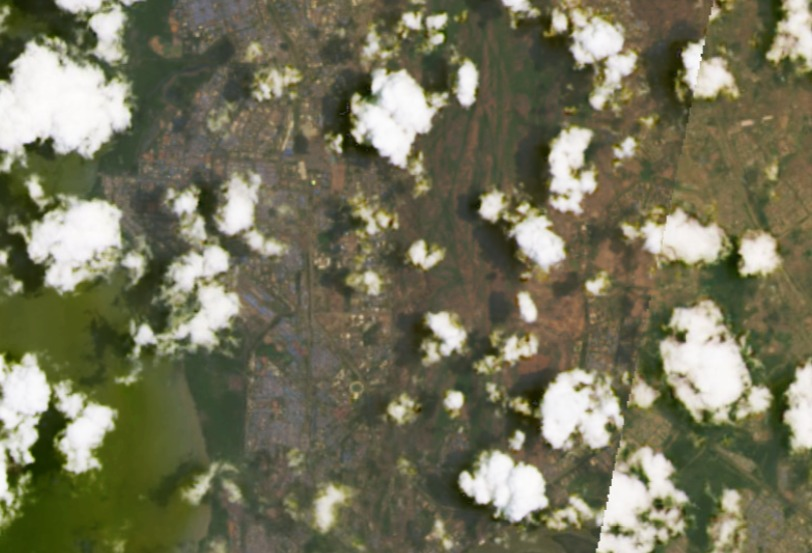
\includegraphics[width=.4\linewidth]{./images/dense.jpeg}
    \hfil
    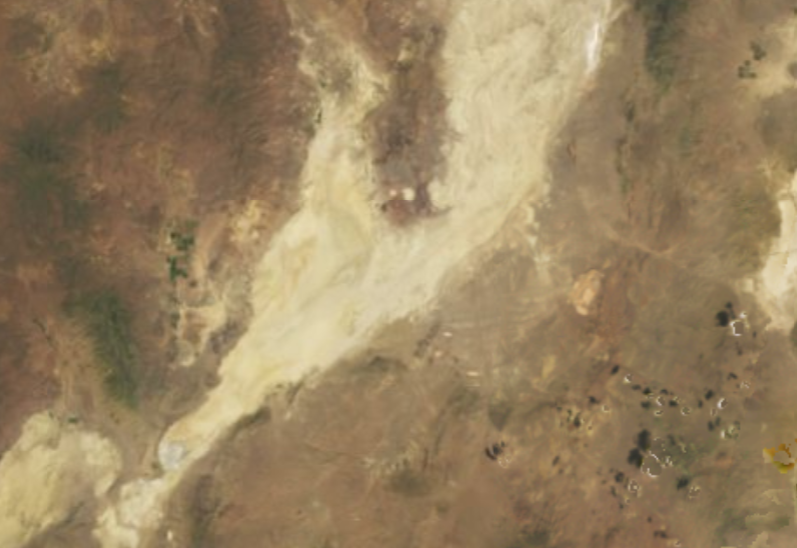
\includegraphics[width=.4\linewidth]{./images/sparse.png}
    \caption{Examples of NASA Landsat satellite images for (a) Densely (b) Sparsely populated regions}
    \label{fig:nasa_images}
\end{figure}

\subsubsection{Creating an ensemble of deep learning and tree-based models} 

We plan to experiment with ensemble learning methods, combining our best-performing and deep-learning models. An ensemble approach could leverage the unique strengths of each model to enhance the overall performance. For instance, while deep learning models excel at extracting high-level features from data, tree-based models can offer more interpretability and are less prone to overfitting. The synergy between these models in an ensemble setup could potentially lead to superior predictive power.


\bibliographystyle{unsrt}
\bibliography{references}

\section{Team contributions}
% Write a brief summary of what each team member did for the project (about 1 or 2 sentences per person). 
\textbf{Debajyoti Dasgupta:} Started with exploratory data analysis and analyzing some models to figure out the best-performing models. Primarily worked with Random Forest Regressor and Deep Neural Networks. Extended on the Random and Grid Search for Random forest regressor hyperparameter tuning. Additionally explored NASA datasets and web scraping to collect image-based data. I also was involved in creating a preliminary CNN-based model and ideation for present and future approaches. Majorly designed, organized, and completed the majority of the report.\\
\\
\textbf{Rushil Venkateswar:} Preformed dataset cleaning and exploration of Dask methodology and other distributed data packages along with the ideation and model creation and testing for XGBoost, TabNet, and Random Forest model. Significantly contributed to the feature reduction step and efficient data storage with parquet-based storage methods. Also worked on performing Grid search and performing hand tuning hyperparameter tuning to improve the performance of the model.\\
\\
\textbf{Piran Karkaria:} Helped with the exploration and detailed description of the dataset and exploring other sources. Provided insights on data cleaning and writing a first draft of the report.

% \appendix

% \section{Appendix (optional)}
% If you wish, you can include an appendix, which should be part of the main PDF, and does not count towards the 6-8 page limit.
% Appendices can be useful to supply extra details, examples, figures, results, visualizations, etc., that you couldn't fit into the main paper. However, your grader \textit{does not} have to read your appendix, and you should assume that you will be graded based on the content of the main part of your paper only.

\end{document}
